\subsection{VPA}
\subsubsection{VPA CPU Utilization}
\begin{itemize}
    \item VPA initially allocates CPU resources based on current requirements but can increase or decrease them dynamically.
    \item As demand changes, VPA adjusts CPU allocations, potentially causing spikes or dips in utilization as resources are adapted.
    \item These adjustments aim to maintain efficient resource usage and consistent application performance.
\end{itemize}

\noindent Below is the graph that illustrates the adjustments in resource allocation for VPA:

\begin{figure}[h]
    \begin{minipage}[t]{0.5\textwidth}
        \centering
        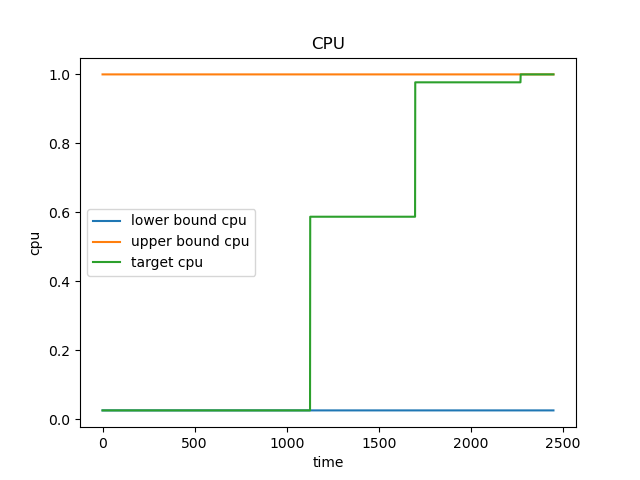
\includegraphics[width=0.9\textwidth]{../sample_results/loop/vpa/cpu-utilization-vpa.png}
        \caption{Loop}
    \end{minipage}
    \hfill
    \begin{minipage}[t]{0.5\textwidth}
        \centering
        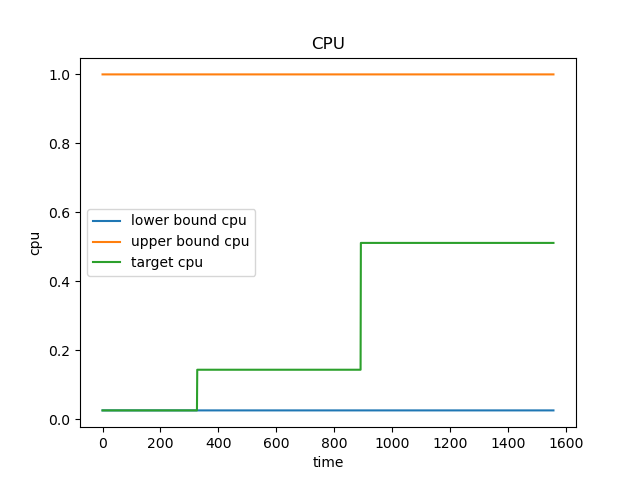
\includegraphics[width=0.9\textwidth]{../sample_results/lorem/vpa/cpu-utilization-vpa.png}
        \caption{Lorem}
    \end{minipage}
\end{figure}
\newpage
\subsubsection{VPA Response Time Observations}
\begin{itemize}
    \item Response times in the VPA configuration can vary as resources are adjusted to meet demand.
    \item Dynamic adjustments in pod resources can lead to fluctuations in response times.
    \item As the VPA optimizes CPU allocations, response times may stabilize, especially when demand is consistent.
    \item VPA aims to balance resource utilization with consistent response times, adapting to varying workloads.
\end{itemize}

\noindent Below are the response time graphs for VPA:

\begin{figure}[h]
    \begin{minipage}[t]{0.5\textwidth}
        \centering
        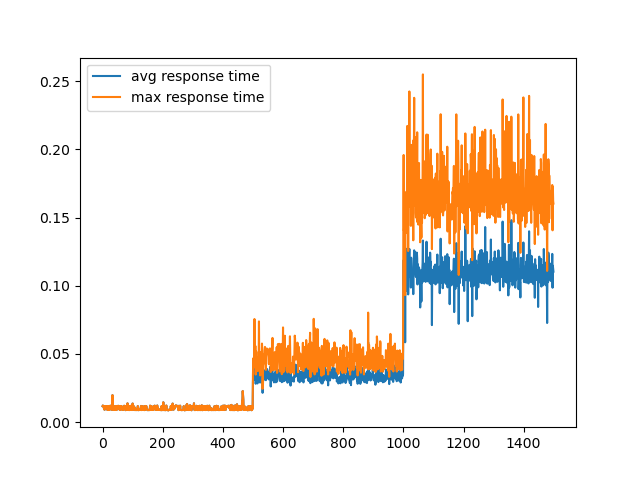
\includegraphics[width=0.9\textwidth]{../sample_results/loop/vpa/response-time-vpa-vpa.png}
        \caption{Loop}
    \end{minipage}
    \hfill
    \begin{minipage}[t]{0.5\textwidth}
        \centering
        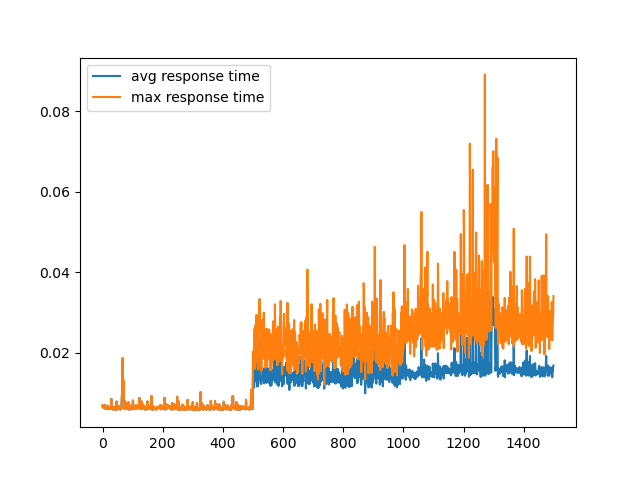
\includegraphics[width=0.9\textwidth]{../sample_results/lorem/vpa/response-time-vpa-vpa.png}
        \caption{Lorem}
    \end{minipage}
\end{figure}

\newpage
\subsubsection{VPA Memory Utilization}
\begin{figure}[h]
    \begin{minipage}[t]{0.5\textwidth}
        \centering
        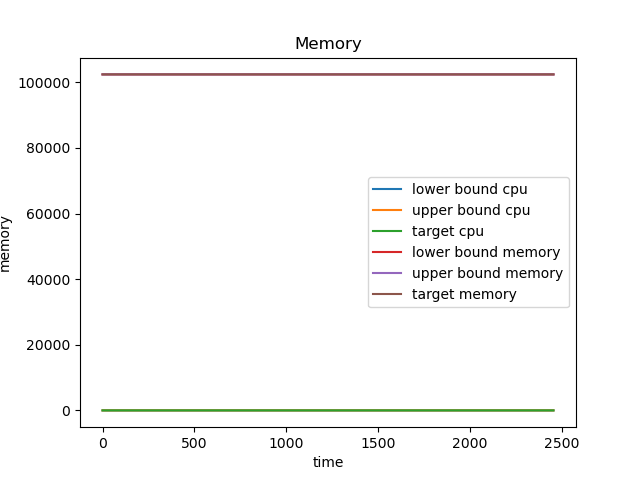
\includegraphics[width=0.9\textwidth]{../sample_results/loop/vpa/mem-utilization-vpa.png}
        \caption{Loop}
    \end{minipage}
    \hfill
    \begin{minipage}[t]{0.5\textwidth}
        \centering
        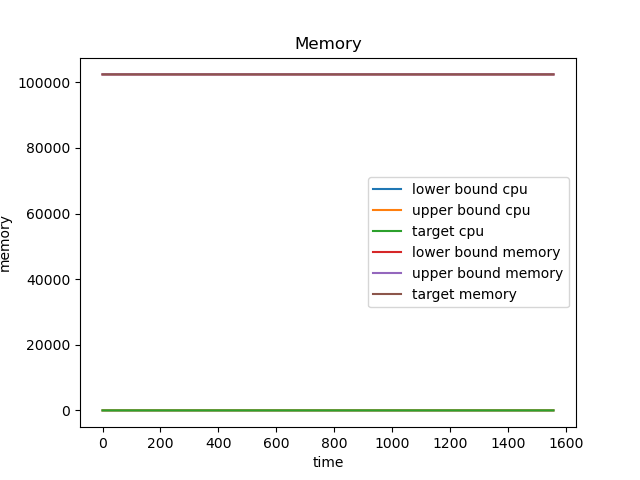
\includegraphics[width=0.9\textwidth]{../sample_results/lorem/vpa/mem-utilization-vpa.png}
        \caption{Lorem}
    \end{minipage}
\end{figure}

\begin{itemize}
    \item VPA manages memory allocations dynamically, adjusting resources according to application needs.
    \item Initial memory usage may vary based on initial resource requests set by VPA.
    \item As the VPA adjusts memory allocations, memory utilization stabilizes according to application requirements.
    \item This adaptive approach optimizes memory usage and aims to maintain consistent application performance.
\end{itemize}

